% FILE: figures/metatheory_k10_selfreference.tex
% K10 meta-theory self-reference schematic

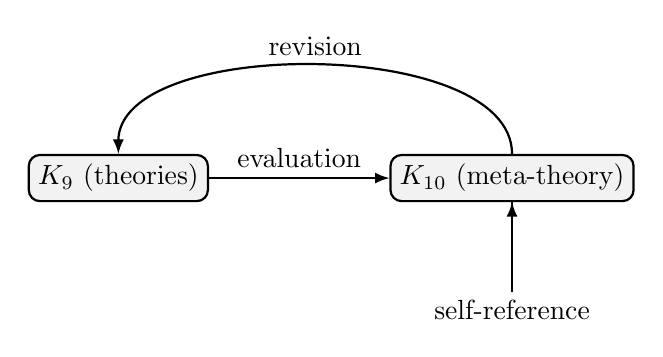
\begin{tikzpicture}[>=latex,thick,scale=1]
  % Nodes
  \node[draw, rounded corners, fill=gray!10] (K9) at (0,0) {$K_9$ (theories)};
  \node[draw, rounded corners, fill=gray!10] (K10) at (5,0) {$K_{10}$ (meta-theory)};

  % Arrows
  \draw[->] (K9) -- node[above] {evaluation} (K10);
  \draw[->] (K10) .. controls (5,1.8) and (0,1.8) .. node[above] {revision} (K9);
  \draw[->] (K10) .. controls (5,-1.8) and (5,-1.8) .. node[below] {self-reference} (K10);
\end{tikzpicture}





